\begin{frame}
\frametitle{Learning network protocols despite imperfect assumptions}
\begin{centering}
Is there a tradeoff between performance and operating range in link rates?
\end{centering}
\end{frame}


\begin{frame}
\frametitle{Performance vs. link-rate operating range}
\begin{centering}

\noindent \only<1>{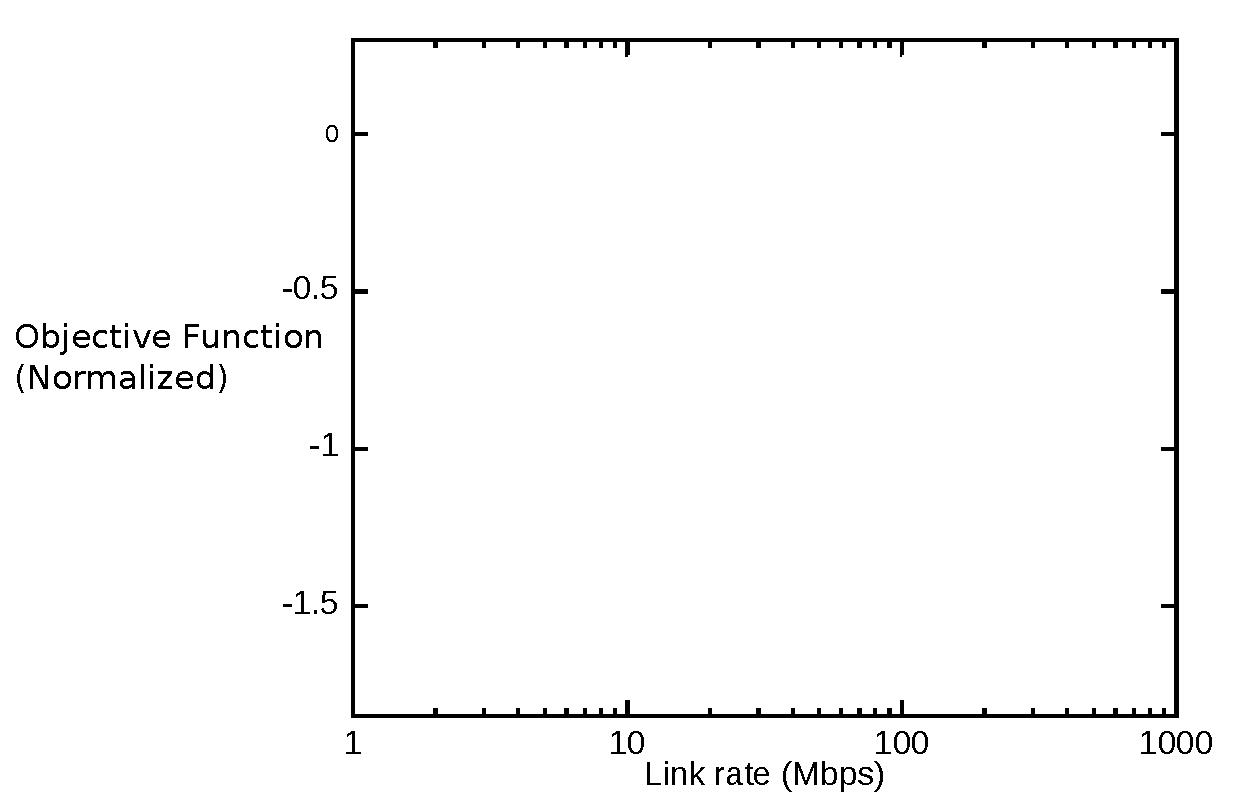
\includegraphics[width=4.1 in]{oprange-base.pdf}}\only<2>{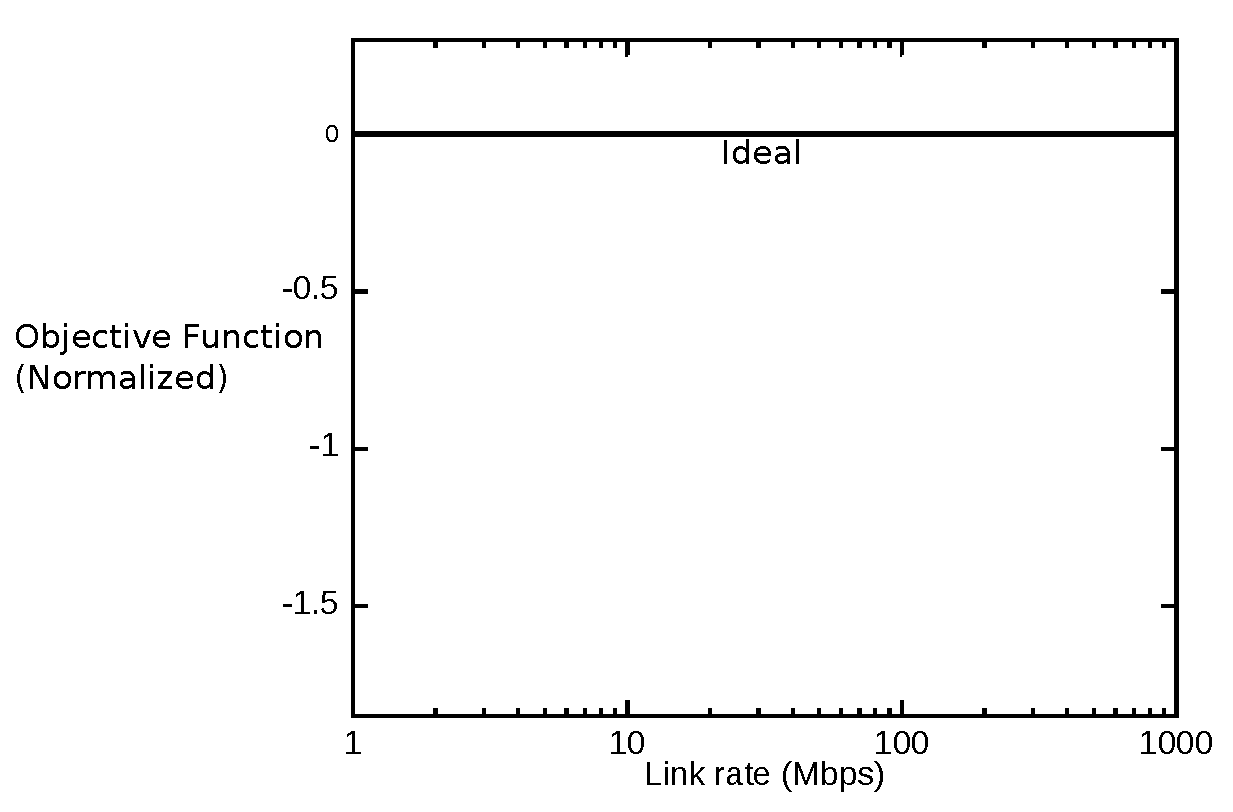
\includegraphics[width=4.1 in]{oprange-omniscient.pdf}}\only<3>{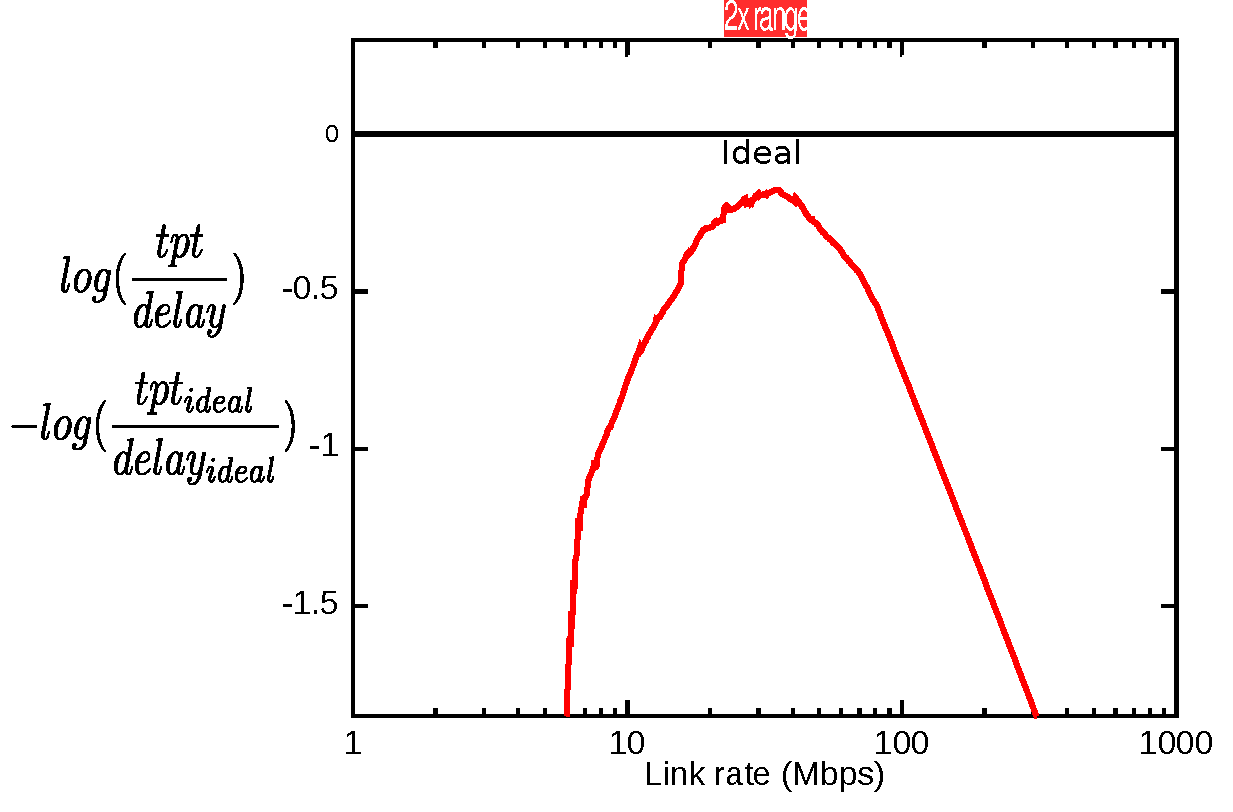
\includegraphics[width=4.1 in]{oprange-2x.pdf}}\only<4>{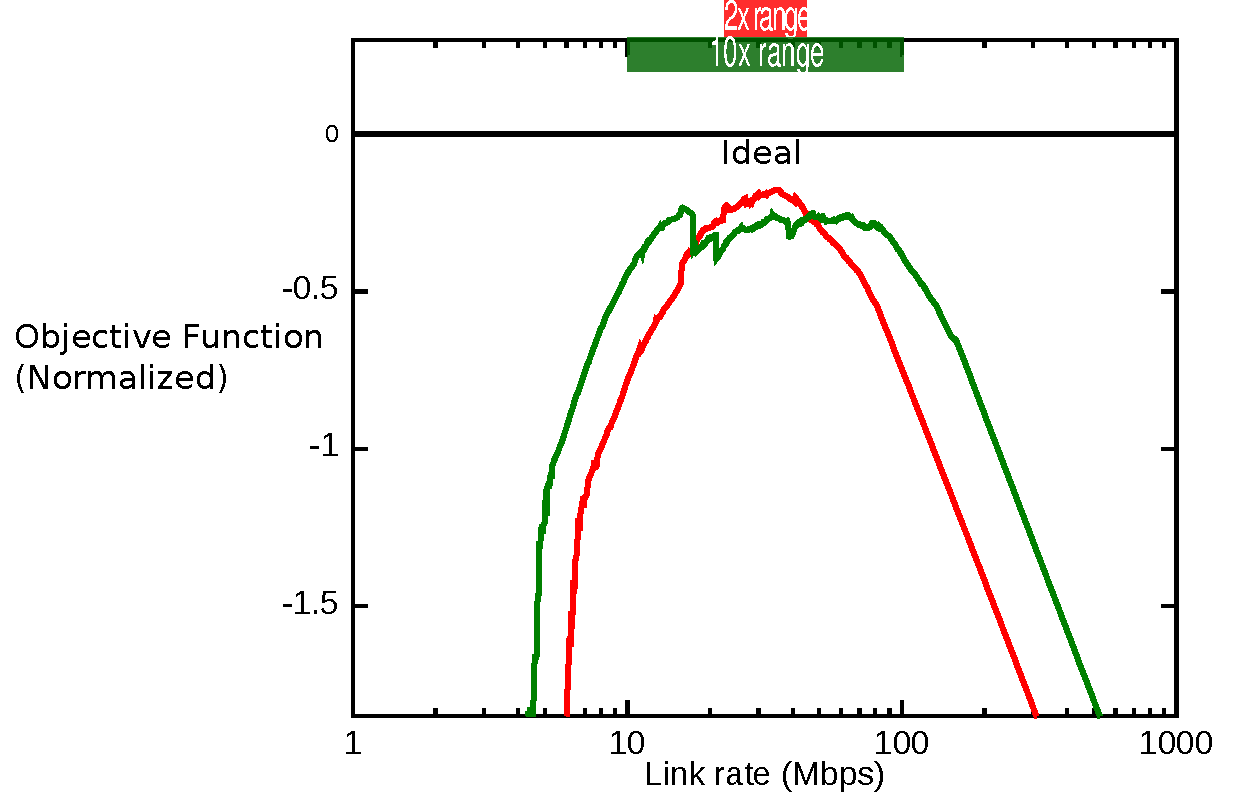
\includegraphics[width=4.1 in]{oprange-10x.pdf}}\only<5>{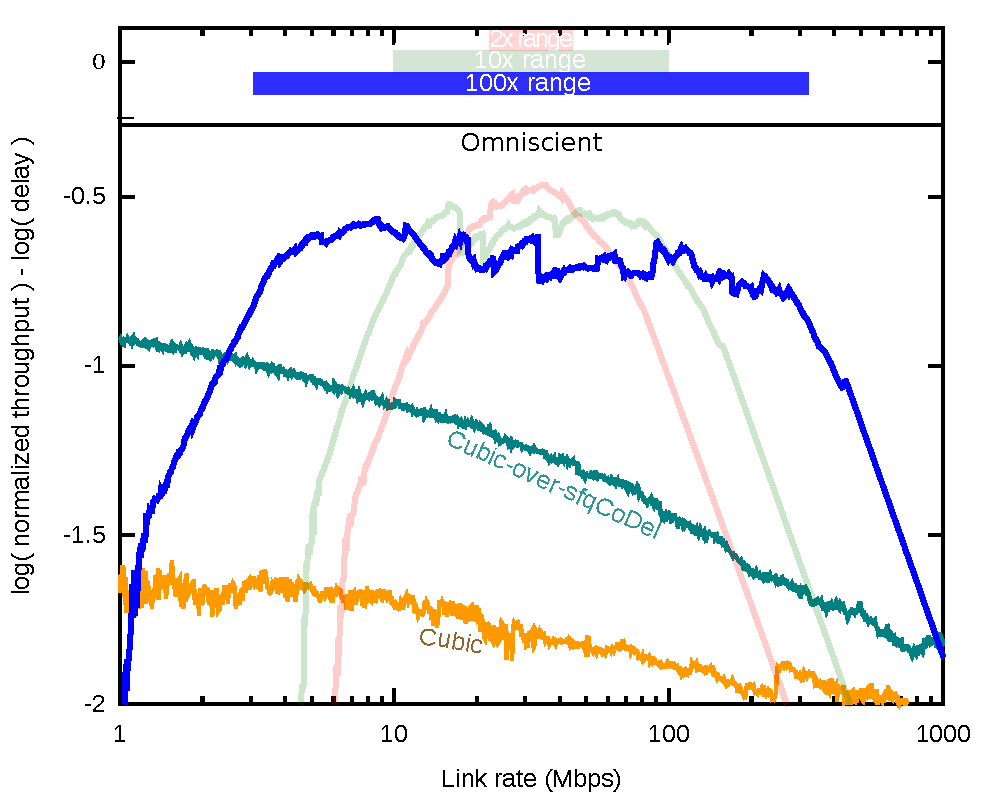
\includegraphics[width=4.1 in]{oprange-100x.pdf}}\only<6>{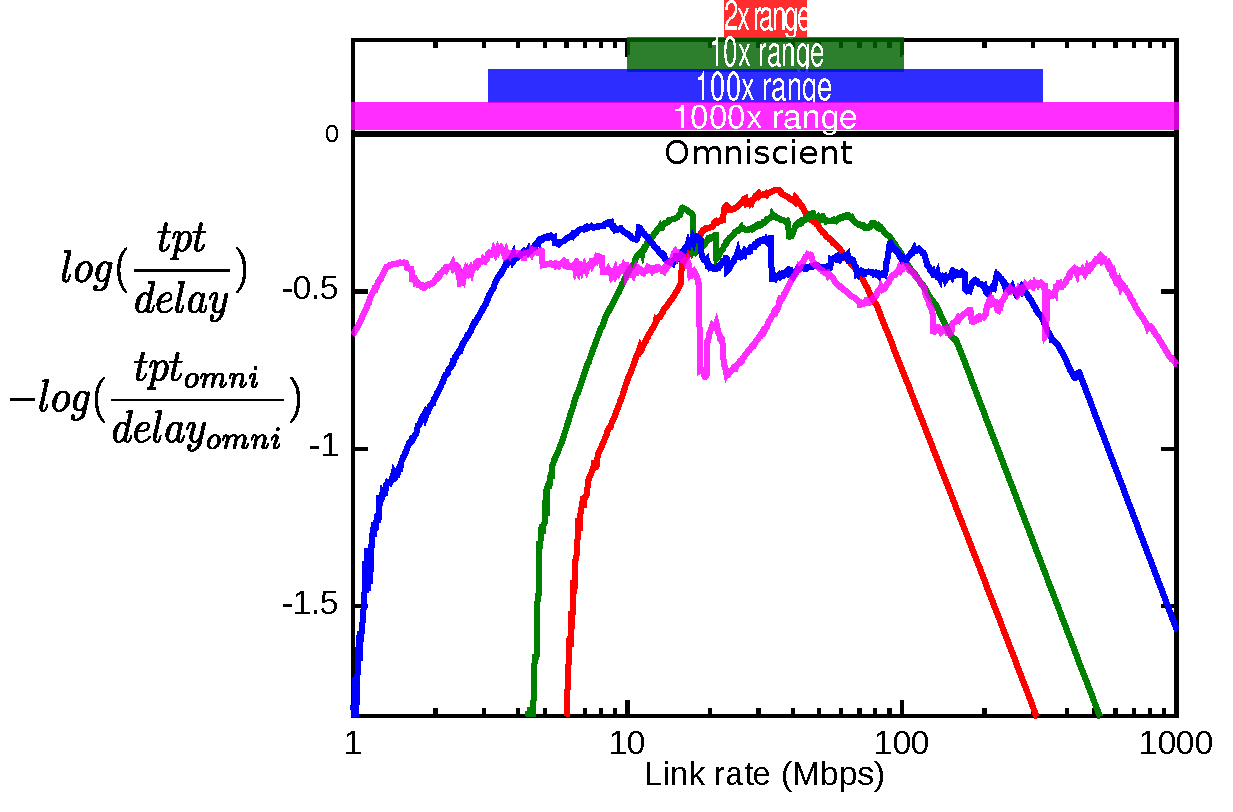
\includegraphics[width=4.1 in]{oprange-1000x.pdf}}\only<7>{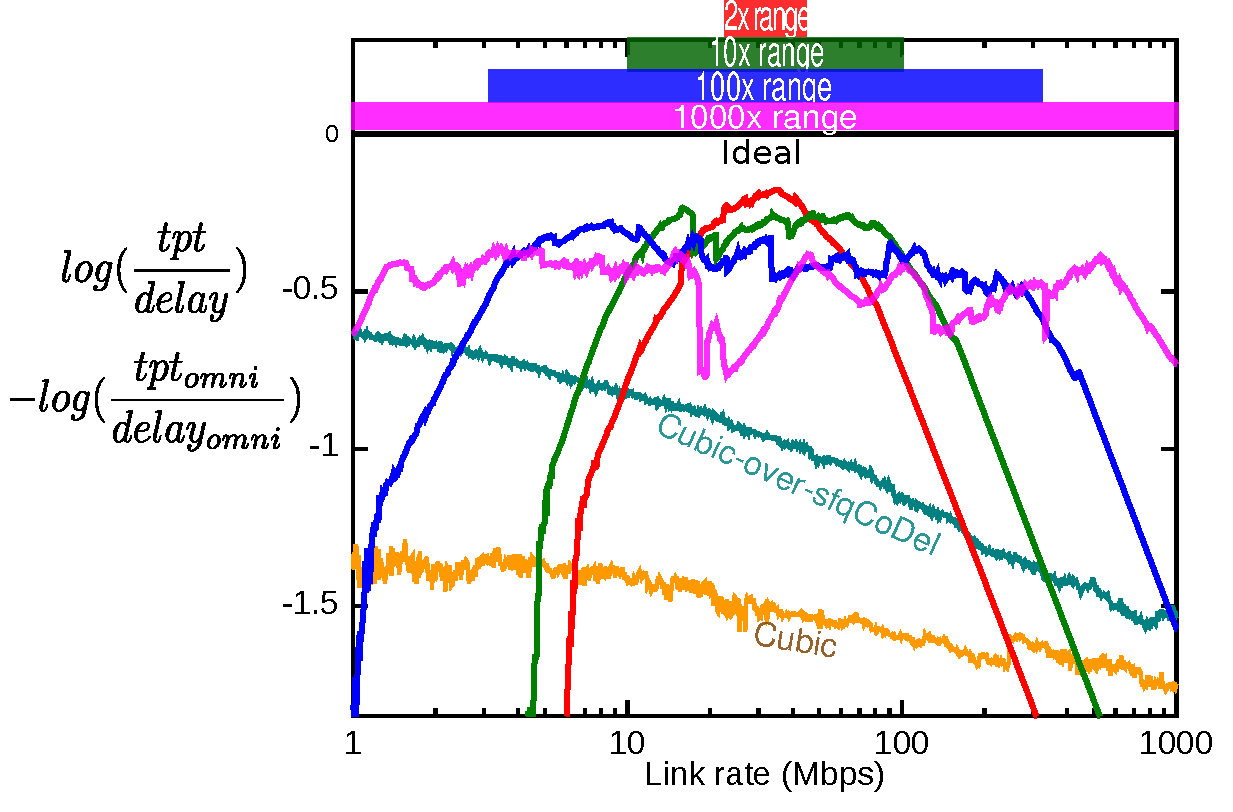
\includegraphics[width=4.1 in]{oprange-rest.pdf}}

\end{centering}
\end{frame}

\begin{frame}
\frametitle{Performance vs. link-rate operating range}
\begin{itemize}
\item <2->{Only weak evidence of a performance-operating range tradeoff}
\item <3->{Possible to design a forwards-comptabible protocol handling a wide range in link rates}
\end{itemize}
\end{frame}
